%second chapter of your thesis
\chapter{Hardware}
Op ons wagentje kun je zien dat we gebruik maken van 3 zelfgemaakte PCB$\prime$s. Twee ervan zijn de combinatie van de Motorshield en de arduino/atmega. De andere is om het overzichtelijk te houden voor de kabels.

\section{Tussenstuk}
We maken gebruik van een tussenstukje, zodat alle line-following sensors naar hetzelfde printplaatje gaan en dit printplaatje dan enkel met 1 voeding en 1 ground moet verbonden worden. De uitgangssignalen worden hier gewoon doorgegeven naar de Atmega. We hebben op dit printplaatje ook de mogelijkheid voorzien om de Bluetooth-module en de RFID-reader aan te sluiten. We hebben nadien ontdekt dat de RFID-reader niet echt kon aangesloten worden op dit printplaatje, om de simpele reden dat het gebruik maakt van dezelfde pinnen die we nodig hebben voor de motoraansturing. Dit leggen we later nog uitgebreider uit. \\
\begin{figure}[h]
\centering
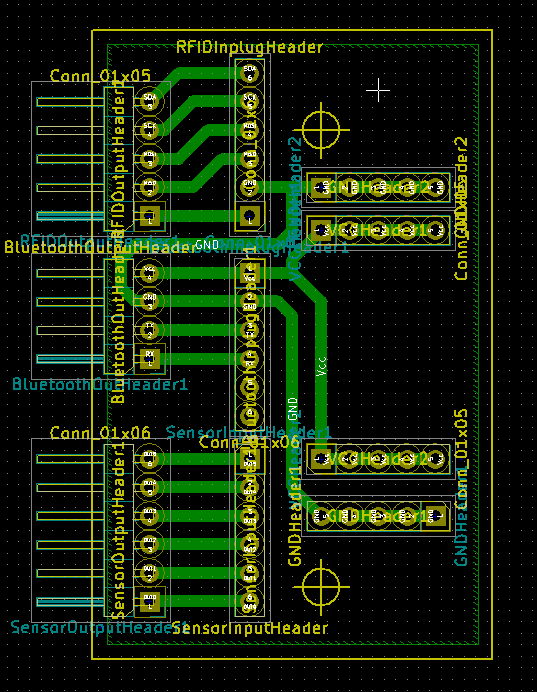
\includegraphics[width=0.75\textwidth]{tussenstukPCB.PNG}
\caption{Routing van de PCB die als verlengstuk dient. \label{tussenstukPCB}}
\end{figure}
We hebben dus 10 5V-aansluitingen voorzien, 10 GND-aansluitingen, de outputs van de sensors die doorgestuurd kunnen worden, de pinnen nodig voor de Bluetooth-module (Key, Vcc, GND, TXD, RXD en State) en de signalen nodig voor de RFID-reader, maar dit wordt niet gebruikt. Niet alle zes de uitgangen van de Bluetooth-module moeten worden doorgestuurd naar onze atmega, deze vereenvoudiging vindt ook plaats op deze PCB. Enkel de signalen Vcc, GND, TXD en RXD worden van een uitgang voorzien. Deze uitgangen worden dus doorverbonden met de Atmega. De Vcc en de GND aan deze uitgang zorgen dus ook voor de voeding van de volledige PCB. We maken gebruik van de HC05 Bluetooth-module, een foto van de module wordt weergegeven in afbeelding~\ref{fig:HC05}.
\begin{figure}[h]
\centering
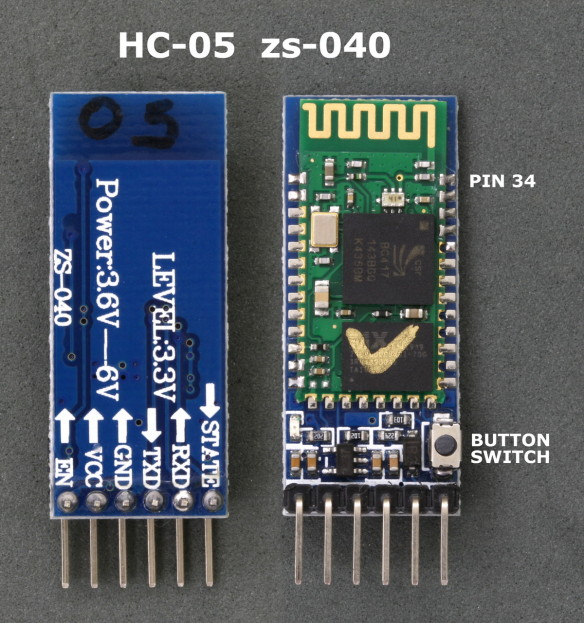
\includegraphics[width=0.75\textwidth]{HC05.jpg}
\caption{De gebruikte Bluetooth-module, ingeplugt op de verlengPCB.}
\label{fig:HC05}
\end{figure}
\section{Ardumoto}
\subsection{Ardumoto RFID}
De tweede printplaat die we gebruiken is eigenlijk ook de volledige combinatie van de atmega en de motorshield, maar we gebruiken enkel de atmega. Deze PCB zorgt voor de aansturing van de RFID-reader. We hebben een tweede atmega nodig omdat de RFID-reader volgende signalen nodig heeft om correct aangestuurd te worden: SS/RX, SCK, MOSI, MISO/TX, IRQ, GND, RST, Vcc. 3 van deze pinnen worden ook gebruikt voor de motoraansturing. SCK is namelijk dezelfde pin als die voor de aansturing van de richting van motor B. MOSI is dezelfde pin als die voor de aansturing van de snelheid van motor B. En de laatste overeenkomstige pin is die van MISO, dit is namelijk dezelfde pin als de aansturing van de richting van motor A. Over deze signalen kunnen er geen twee signalen tergelijkertijd worden over gestuurd. We konden ook eventueel gebruik maken van het $I^{2}C$ principe, in plaats van ISP. Door $I^{2}C$ te gebruiken gingen we geen pinnen nodig hebben die we al gebruikt hadden en dus ook geen tweede PCB, maar we waren toen al beter aan een wat verbeterde versie van de PCB waardoor we dus toch twee werkende PCB$\prime$s gingen hebben. We hadden ook al een werkende code voor de RFID gebasseerd op het ISP protocol. We hebben gebruik gemaakt van een RFID-reader-module, nl. de MRFC522, deze module wordt weergegeven in figuur~\ref{fig:MRFC522}. Om een RFID uit te lezen moet de reader op $\approx$ 1 cm passeren boven de tag. Dit probleem hebben we opgelost door een stukje te laten printen die we vastvijzen aan het wagentje.
\begin{figure}[h]
\centering
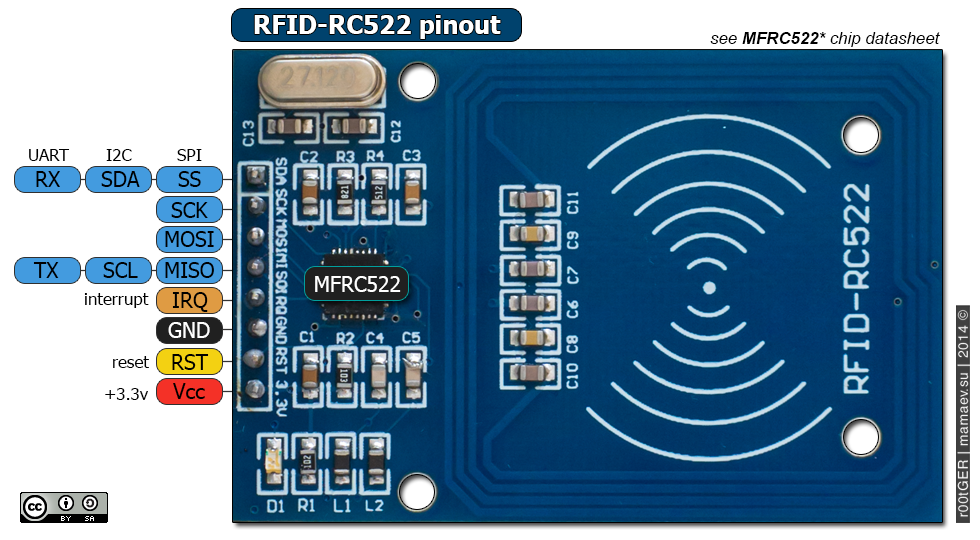
\includegraphics[width=0.75\textwidth]{MRFC522.png}
\caption{Gebruikte RFID-reader MRFC522. \label{fig:MRFC522}}
\label{fig:ACEquiv}
\end{figure}
\subsection{Ardumoto Motor}
Deze PCB dient voor de aansturing van de motoren en ook het doorsturen van de signalen naar de Raspberry Pi via de Bluetooth module. Er waren nog enkele fouten gekropen in het PCB-design. Enkele footprints waren aan de kleine kant, terwijl we dachten na de eerste keer we ze wat aangepast hadden. Maar de grootste fout die erin zat was dat we een ingang van de L298 (de IC verantwoordelijk voor de motoraansturing) vergeten te verbinden waren met het PWRIN signaal. \\
Als basis van ons schema hebben we gebruik gemaakt van een Arduino Uno. Om te beginnen konden we de USB interface voor de aansluiting van een USB-kabel weglaten. (FOTO USB) Dit konden we weglaten doordat we gebruik gingen maken van de ICSP-pinnen mbv. een andere Arduino. We hebben ook bewust alle LED$\prime$s weggelaten omdat we dit niet echt nodig hebben en dit onze arduino groter zou maken dan strikt nodig. We hebben ook de labels verandert van het standaardschema naar wat meer betekenisvolle namen zoals bijvoorbeeld MISO vervangen door DIR A. (FOTO ATMEGA) R8 bijvoorbeeld hebben we ook weggelaten, deze weerstand wordt vaak gebruikt om een brugje te cre$\ddot{e}$ren om baantjes te kunnen ondertrekken. Pinnen 27 en 28 hebben we niet nodig, dus mogen we de condensator hier rond ook verwijderen. De jumper hebben we weggelaten omdat we die niet nodig achtten. 

%In het vorig hoofdstuk hebben we naar deze tekst verwezen\label{verwijzing}.
